Per collegare l'architettura al comportamento osservabile, il capitolo segue
alcune richieste dall'ingresso in \emph{Copernicus Data Workspace} fino alla
risposta. Gli scenari sono ricavati dal comportamento implementato e i valori
citati hanno scopo illustrativo. I risultati di benchmark sono presentati nel
Capitolo~\ref{cap:7}.

\section{Ingresso della richiesta}

Dalla home del workspace l'utente descrive luogo, fenomeno e periodo e avvia
una nuova analisi; può anche riprendere un'indagine precedente che conserva
dashboard, filtri e contesto. La dashboard invia i messaggi al backend mediante
l'endpoint compatibile con le chat completion OpenAI. La richiesta contiene
modello, cronologia, opzione di streaming e i metadati da cui si ricava
l'identificativo della conversazione. Il backend normalizza tale
identificativo e avvia il workflow.

Nel client legacy Open WebUI compaiono anche richieste tecniche generate
dall'interfaccia (titolo della chat, suggerimenti), che il sistema riconosce e
gestisce separatamente dalle domande geografiche.

Il primo nodo del workflow estrae l'ultimo messaggio dell'utente e lo ripulisce
dai marcatori dell'interfaccia. Il Gateway decide quindi come procedere. Da
questo punto sono possibili tre casi:

\begin{enumerate}
    \item nuova richiesta ammessa: parsing e routing completi;
    \item follow-up ammesso: riuso del checkpoint e selezione dei soli nodi
    necessari;
    \item richiesta fuori dominio o classificazione fallita: risposta diretta.
\end{enumerate}

\section{Scenario 1: analisi multi-sorgente di un pericolo}

Si consideri la domanda:

\begin{quote}
\emph{``Mostrami i terremoti di magnitudo superiore a 4,5 avvenuti in Italia
negli ultimi sette giorni e fammi vedere la copertura satellitare.''}
\end{quote}

\subsection{Risoluzione semantica}

Il parser produce una richiesta strutturata simile alla seguente:

\begin{itemize}
    \item categoria: pericolo, sottotipo terremoto;
    \item luogo: Italia, con bounding box quando il geocoding è disponibile;
    \item periodo: intervallo assoluto corrispondente agli ultimi sette giorni;
    \item filtro: magnitudo maggiore di 4,5;
    \item viste: dati strutturati e mappa.
\end{itemize}

Il riferimento temporale viene risolto in date precise rispetto all'istante
corrente e al fuso orario del backend; il luogo viene trasformato, quando
possibile, da etichetta a geometria.

\subsection{Pianificazione ed esecuzione}

Poiché la categoria è un pericolo, il piano comprende Search, GDACS e
Copernicus STAC. I tre worker partono in parallelo:

\begin{itemize}
    \item Search recupera contesto web attuale;
    \item GDACS chiede al server MCP gli eventi e applica i filtri;
    \item STAC interroga CDSE per area, periodo e collezioni.
\end{itemize}

Il filtro GDACS richiede che periodo, magnitudo, tipo e posizione siano
soddisfatti dallo stesso record. Se sono presenti coordinate, la verifica
spaziale usa la bounding box del luogo oltre al nome del paese. Una bounding
box nazionale è un rettangolo e può includere aree confinanti: funziona quindi
come filtro geometrico. Per una richiesta cittadina il sistema mantiene
l'ambito della città. La risposta riporta gli eventi presenti nel feed
interrogato.

Il client STAC invia una ricerca con bounding box e intervallo ISO 8601. Per
intervalli o aree estesi può suddividere la richiesta in partizioni temporali
e quadranti, con un numero limitato di tentativi. I risultati sono ridotti ai
metadati utili e deduplicati per identificativo. Il client legge soltanto la
prima pagina di risultati di ciascuna ricerca: per aree o periodi molto ampi
i conteggi si riferiscono quindi ai prodotti recuperati, che possono essere
meno di quelli presenti nel catalogo.

\subsection{Sincronizzazione e risposta}

LangGraph attende la convergenza dei worker. Il Chart Agent riceve soltanto
dataset normalizzati e aggregazioni; il renderer della mappa riceve bounding
box e relativi centri. Le acquisizioni STAC alimentano inoltre un artefatto
dashboard incorporato nel workspace. Il Conversation Agent compone infine:

\begin{enumerate}
    \item sintesi testuale;
    \item eventuali tabelle;
    \item dashboard Copernicus con KPI, grafici, tabella e heatmap;
    \item elenco delle fonti consultate.
\end{enumerate}

\begin{figure}[htbp]
\centering
\resizebox{0.96\textwidth}{!}{%
\begin{tikzpicture}[
    actor/.style={rectangle,draw=black!70,fill=blue!8,minimum width=24mm,
        minimum height=8mm,align=center},
    msg/.style={-{Latex[length=2mm]},thick},
    return/.style={-{Latex[length=2mm]},thick,dashed},
    every node/.style={font=\small}
]
    \node[actor] (u) at (0,0) {Utente};
    \node[actor] (a) at (3.2,0) {API};
    \node[actor] (w) at (6.4,0) {Workflow};
    \node[actor] (s) at (9.6,0) {Sorgenti};
    \node[actor] (v) at (12.8,0) {Vista};

    \foreach \x in {0,3.2,6.4,9.6,12.8}
        \draw[gray!60] (\x,-0.5) -- (\x,-6.8);

    \draw[msg] (0,-1.0) -- node[above]{domanda} (3.2,-1.0);
    \draw[msg] (3.2,-1.8) -- node[above]{messaggi + thread} (6.4,-1.8);
    \draw[msg] (6.4,-2.6) -- node[above]{query strutturate} (9.6,-2.6);
    \draw[return] (9.6,-3.5) -- node[above]{dataset normalizzati} (6.4,-3.5);
    \draw[msg] (6.4,-4.4) -- node[above]{artefatti} (12.8,-4.4);
    \node[align=center,font=\scriptsize] at (12.8,-5.2)
        {rendering\\nel browser};
    \draw[return] (6.4,-6.0) -- node[above]{risposta finale} (3.2,-6.0);
    \draw[return] (3.2,-6.6) -- node[above]{stream SSE} (0,-6.6);
\end{tikzpicture}}
\caption{Sequenza end-to-end di una richiesta multi-sorgente. Il workflow
costruisce l'artefatto dashboard a partire dai record STAC normalizzati; il
browser lo carica e lo presenta così com'è.}
\label{fig:sequenza-end-to-end}
\end{figure}

\section{Scenario 2: interrogazione di una attivazione CEMS}

La domanda:

\begin{quote}
\emph{``Dammi i dettagli dell'attivazione Copernicus EMSR884.''}
\end{quote}

contiene un identificativo univoco. Il ramo CEMS risponde alla domanda
diretta; nel prototipo il piano può attivare anche Search e STAC come
\emph{arricchimento} per contesto e dashboard. Si tratta di una scelta di
prodotto, che aggiunge latenza e dipendenze rispetto alla sola richiesta di
dettaglio. Il CEMS Router valida il codice nel formato \texttt{EMSR\#\#\#} o
\texttt{EMSN\#\#\#} e sceglie l'endpoint corretto.

Per \texttt{EMSR} vengono consultati i dettagli Rapid Mapping; per
\texttt{EMSN} quelli Risk and Recovery. Il dataset restituito può includere
paese, categoria, stato, istante di attivazione, aree di interesse, numero e
tipo dei prodotti, URL di download o mappe.

Se una domanda successiva chiede anche le acquisizioni Sentinel nella medesima
area, il ramo CEMS viene eseguito prima di STAC e le coordinate
dell'attivazione guidano direttamente la ricerca satellitare.

\section{Scenario 3: follow-up e riuso della memoria}

Dopo una prima risposta l'utente può scrivere:

\begin{quote}
\emph{``Ora raggruppali per giorno e mostrami un grafico a barre.''}
\end{quote}

Il messaggio dipende dal contesto. Nell'esempio l'artefatto selezionato è
quello delle acquisizioni STAC; se il turno precedente conteneva anche eventi
GDACS, il sistema lavora sul dataset attivo nella conversazione; per
raggruppare un altro dataset l'utente lo indica esplicitamente. Il Gateway riceve una vista compatta dello stato e riconosce la
continuità del dominio. Il Conversation Agent sceglie quindi una delle azioni
di follow-up:

\begin{itemize}
    \item risposta basata sui dati già presenti;
    \item nuovo grafico o nuova heatmap dello stesso dataset;
    \item aggiornamento di una singola sorgente;
    \item aggiornamento di più sorgenti;
    \item nuova richiesta, se l'utente cambia oggetto.
\end{itemize}

Nell'esempio il Chart Agent usa il dataset conservato in Redis e aggiorna la
visualizzazione, senza ripetere le chiamate GDACS e STAC. Se l'utente opera
nella dashboard, il Composer traduce il comando in una mutazione tipizzata e
il backend salva una nuova revisione dell'artefatto. Il riuso risparmia
chiamate alle sorgenti e il relativo traffico; il guadagno sui tempi
richiederebbe una misura controllata. Quando l'utente chiede informazioni
correnti, il sistema aggiorna esplicitamente le fonti.

\begin{figure}[htbp]
\centering
\begin{tikzpicture}[
    node distance=9mm and 12mm,
    flowbox/.style={rectangle,rounded corners,draw=blue!65!black,thick,
        fill=blue!10,align=center,minimum height=9mm,text width=27mm},
    decision/.style={diamond,aspect=2,draw=violet!65!black,thick,
        fill=violet!10,align=center,text width=22mm,inner sep=1pt},
    line/.style={-{Latex[length=2mm]},thick}
]
    \node[flowbox] (follow) {Nuovo turno};
    \node[decision,right=of follow] (ctx) {Contesto sufficiente?};
    \node[flowbox,above right=10mm and 13mm of ctx] (answer) {Rispondi o crea vista\\dal checkpoint};
    \node[flowbox,below right=10mm and 13mm of ctx] (refresh) {Aggiorna solo\\le fonti richieste};
    \node[flowbox,right=28mm of ctx] (compose) {Componi risposta};
    \draw[line] (follow) -- (ctx);
    \draw[line] (ctx) -- node[above left,font=\scriptsize]{si} (answer);
    \draw[line] (ctx) -- node[below left,font=\scriptsize]{no} (refresh);
    \draw[line] (answer) -- (compose);
    \draw[line] (refresh) -- (compose);
\end{tikzpicture}
\caption{Scelta fra riuso della memoria e aggiornamento delle fonti.}
\label{fig:follow-up}
\end{figure}

\section{Scenario 4: scoprire un dataset nel grafo}
\label{sec:scenario-discovery}

Si consideri la richiesta:

\begin{quote}
\emph{``Cerco un dataset orario di temperatura superficiale del Mar Nero:
quale variabile contiene?''}
\end{quote}

Il Gateway riconosce un compito di Discovery. Il nodo d'intento rappresenta il
tema temperatura superficiale, l'area Mar Nero, la risoluzione oraria e il
tipo dataset con variabile. Il servizio recupera candidati dal sottografo
Marine, ne verifica la compatibilità e applica il ranking deterministico
descritto nella Sezione~\ref{subsec:discovery-workflow}.

Lo snapshot di riferimento del benchmark, salvato il 13 ottobre 2026 e riportato
nella guida \cite{guidaProgetto2026}, associa questa ricerca al dataset
\path{cmems_obs-sst_blk_phy-sst_nrt_diurnal-oi-0.0625deg_PT1H-m}, dal titolo
\emph{Black Sea Diurnal Subskin SST Analysis, L4, 1/16deg hourly}, con variabile
\texttt{analysed\_sst}. La bounding box registrata è
$[26{,}375; 38{,}75; 42{,}375; 48{,}8125]$ nell'ordine ovest, sud, est, nord.
Si tratta di metadati del catalogo, utili a individuare la fonte.

La risposta presenta dataset, variabile e provenienza, e l'artefatto permette
di consultare le risorse selezionate. La scoperta della fonte scientifica
resta così distinta dalla ricerca di scene satellitari; l'analisi dei valori
della variabile è fuori dal perimetro del prototipo.

Se un turno successivo chiede le acquisizioni relative alla stessa area, il
passaggio al percorso operativo conserva il riferimento geografico. Per
verificarlo occorre confrontare intento, query effettiva, artefatto salvato e
viste mostrate nel browser; questo controllo conversazionale è distinto dai
casi a thread nuovo del benchmark.

\section{Dashboard Copernicus}

La dashboard analitica è il canale principale per le visualizzazioni delle
acquisizioni satellitari. Nel ramo operativo viene aperta nel workspace come
artefatto a sé (vista ``Analisi dati Copernicus''), con navigazione dedicata a
risultato, grafici, mappa, dati e attività, più una chat laterale sul
risultato già caricato. Grafici, KPI, tabella e heatmap usano esclusivamente
record STAC Copernicus normalizzati; Search, GDACS e CEMS compaiono nella
risposta testuale o in sezioni separate. In questo modo, per esempio, il
numero di eventi GDACS e il numero di prodotti satellitari restano separati.

\begin{figure}[htbp]
\centering
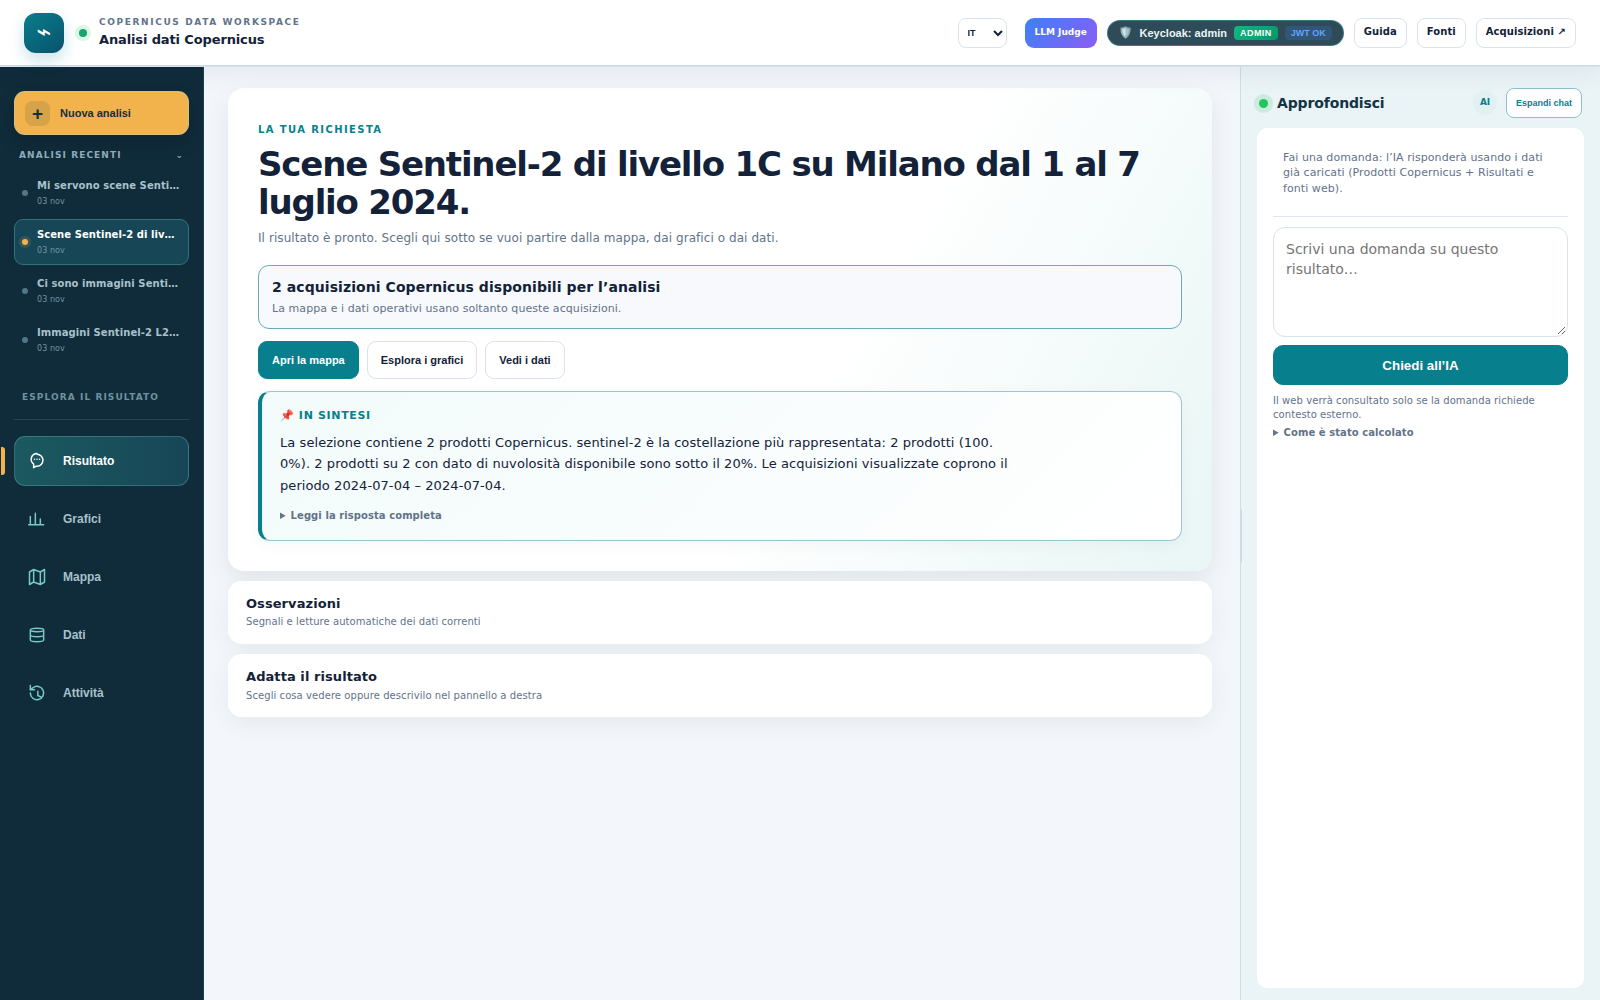
\includegraphics[width=0.92\textwidth]{Images/screenshots/ui-workspace-session.png}
\caption{Sessione operativa ripresa dal workspace: sintesi delle acquisizioni
(conteggio di prodotti/item STAC recuperati), navigazione
Risultato/Grafici/Mappa/Dati e chat laterale sul risultato già caricato.}
\label{fig:ui-workspace-session}
\end{figure}

Il ramo Discovery presenta invece un artefatto del catalogo, con schede e
metadati delle risorse pertinenti. Le due viste rispondono a compiti diversi e
indicano ciascuna la propria provenienza.

\subsection{Dati, provenienza e composizione}

Il Chart Agent costruisce una specifica JSON con valori derivati dal dataset:
etichette, serie, tipo di grafico, campo e misura di origine, filtri, numero di
record e identificativi dei prodotti. Il modello può proporre il tipo di vista
o una nuova aggregazione, mentre conteggi, percentuali, medie, variazioni e
confronti sono sempre calcolati dal backend. La sezione ``Come è stato
calcolato'' e la tabella dei dati di ciascun grafico rendono ispezionabile
questa provenienza; i dati possono inoltre essere esportati in CSV.

La composizione iniziale segue gli output richiesti: una domanda come ``solo
la heatmap'' apre soltanto la mappa, mentre una richiesta generale include
KPI, grafici, tabella, sintesi e mappa. In assenza di acquisizioni l'artefatto
mostra uno stato vuoto esplicito.

\subsection{Grafici leggibili e senza sovrapposizioni}

Le regole di rendering descritte nella
Sezione~\ref{subsec:leggibilita-grafici} vengono applicate alla specifica
generata prima che la dashboard sia mostrata. Il Dashboard Validator riallinea
etichette, valori e serie e intercetta valori non numerici; ECharts gestisce poi
dimensioni, etichette e scorrimento nel browser. La verifica dei dati resta
così separata dalle correzioni puramente grafiche.

\subsection{Interazione, revisioni e chat contestuale}

Nel workspace i controlli visivi permettono di scegliere barre, linee o torta,
ordinamento, Top~N e visibilità dei grafici. Un click su categoria o cella può
attivare un cross-filter: il backend applica il filtro ai record e ricalcola
simultaneamente KPI, grafici, tabella e heatmap. I filtri attivi sono mostrati
e possono essere azzerati con un solo comando.

Ogni modifica passa attraverso azioni tipizzate, validate e salvate. Sono
disponibili annullamento, ripristino e confronto tra revisioni. La chat
contestuale sul risultato ha un thread indipendente per grafico, tabella,
heatmap o dashboard: risponde sul sottoinsieme corrente e trasforma
istruzioni come ``filtra solo Sentinel-2A'' o ``cambia questo grafico in
linee'' in modifiche dell'artefatto. La ricerca web interviene solo quando
serve un contesto esterno ai dati visualizzati. La home del workspace conserva
inoltre l'elenco delle indagini recenti, così da riprendere una sessione senza
ripetere la domanda iniziale.

\subsection{Heatmap Copernicus}

Leaflet rappresenta una heatmap della densità dei centri delle bounding box
degli item recuperati e la collega a una vista con i rettangoli delle bounding
box e i metadati STAC. La heatmap descrive quindi dove si concentrano le
acquisizioni, e non la copertura areale o l'intensità del fenomeno. Se un
cross-filter è attivo, la mappa usa lo stesso sottoinsieme di record degli
altri componenti.

\begin{figure}[htbp]
\centering
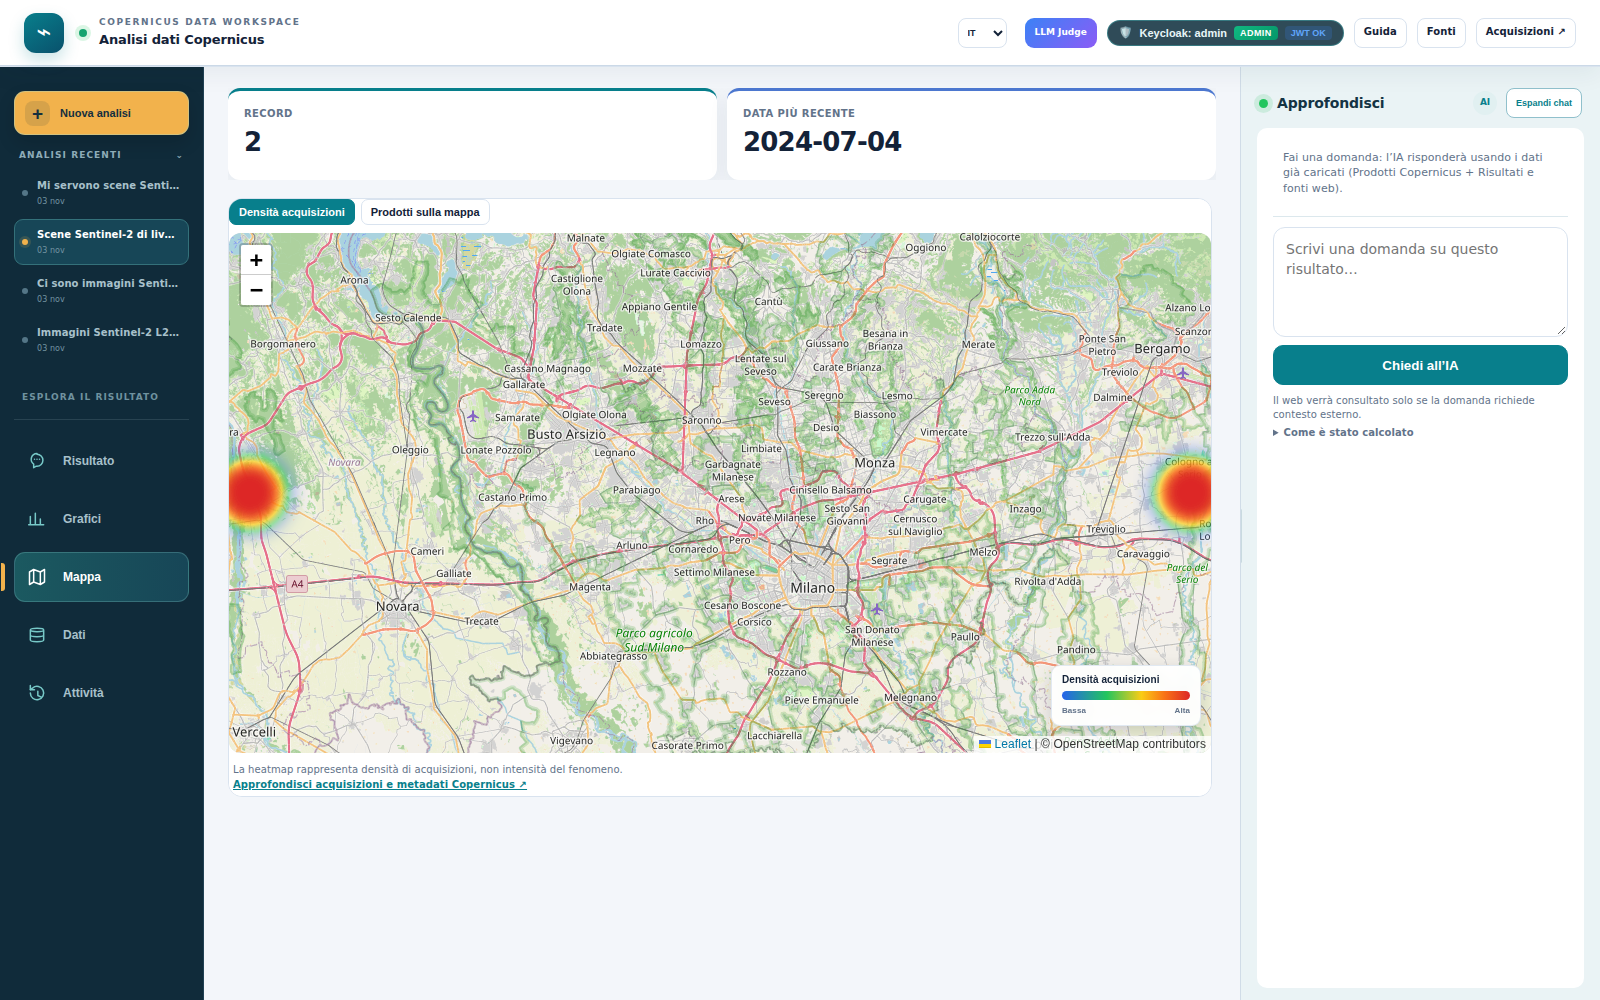
\includegraphics[width=0.92\textwidth]{Images/screenshots/ui-workspace-mappa.png}
\caption{Vista \emph{Mappa}: densità dei centri delle bounding box degli item
STAC recuperati e chat laterale sul risultato.}
\label{fig:ui-workspace-mappa}
\end{figure}

\section{Streaming della risposta}

Durante l'esecuzione il backend invia aggiornamenti sullo stato delle fasi
(interpretazione, routing, recupero delle fonti, composizione). FastAPI
traduce gli eventi LangGraph in Server-Sent Events nel formato delle chat
completion OpenAI; il workspace li mostra come avanzamento della richiesta.

Il testo generato dal Conversation Agent viene rifinito prima della consegna:
tabelle Search/GDACS, fonti e dashboard Copernicus sono aggiunte in un ordine
stabile. Lo stream pubblica la versione finale completa di artefatto e si
chiude con un marcatore di fine.

\section{Gestione degli errori}

\subsection{Errore di una sorgente}

Ogni chiamata a una sorgente segue un contratto di errore comune. Se GDACS
fallisce mentre Search e STAC terminano correttamente, il grafo conserva i
risultati disponibili e il Conversation Agent produce una risposta parziale
che indica con precisione la fonte mancante.

Anche all'interno di STAC una ricerca partizionata può fallire soltanto per
alcune aree o finestre temporali. I prodotti ottenuti restano utilizzabili e
la copertura incompleta viene segnalata nella risposta e nell'artefatto.

Gli errori sono classificati in configurazione, autenticazione, rete, timeout,
risposta non valida e persistenza. A ciascuno sono associati:

\begin{itemize}
    \item codice pubblico stabile;
    \item identificativo diagnostico univoco;
    \item servizio coinvolto;
    \item indicazione sulla possibilità di ripetere l'operazione;
    \item dettaglio tecnico destinato soltanto ai log.
\end{itemize}

\subsection{Timeout e retry}

I retry sono riservati agli errori presumibilmente transitori, come timeout,
problemi di rete, HTTP 429 e HTTP 5xx. Anche il modello remoto dispone di
timeout, backoff e limite di concorrenza, così che i rami paralleli restino
entro la capacità del runner Ollama.

\subsection{Errore della memoria}

Redis è una dipendenza obbligatoria: senza memoria un follow-up potrebbe
sembrare valido pur avendo perso il contesto precedente. Per questo il
servizio si dichiara pronto solo quando memoria e grafo sono disponibili.

\section{Matrice dei percorsi e delle evidenze}

La Tabella~\ref{tab:matrice-percorsi} collega percorsi tipici alle fonti
previste. La Tabella~\ref{tab:funzionalita-evidenza} indica, per le
funzionalità descritte nel capitolo, il tipo di evidenza disponibile: il
benchmark del Capitolo~\ref{cap:7} copre i casi di ricerca nel grafo e di
acquisizioni, mentre GDACS, CEMS, follow-up, autenticazione e ripresa della
sessione sono documentati da test e scenari.

\begin{table}[htbp]
\centering
\small
\begin{tabularx}{\textwidth}{
    >{\bfseries\raggedright\arraybackslash}p{0.25\textwidth}
    >{\raggedright\arraybackslash}p{0.23\textwidth}
    >{\raggedright\arraybackslash}X}
\toprule
Richiesta & Rami principali & Risultato atteso \\
\midrule
Clima in Sicilia &
Piano operativo &
Contesto web e acquisizioni secondo il piano, senza stime climatiche dai raster. \\
\addlinespace
Dataset orario SST del Mar Nero &
Discovery su NebulaGraph &
Risorsa Marine, variabile e metadati di compatibilità. \\
\addlinespace
Siccità in Sicilia e acquisizioni &
Discovery + operativo &
Risorse Drought pertinenti e acquisizioni STAC nella stessa sessione. \\
\addlinespace
Terremoti in Indonesia &
Search + GDACS + STAC &
Eventi filtrati, contesto web e copertura delle acquisizioni. \\
\addlinespace
Dettagli EMSR884 &
CEMS + Search/STAC &
Attivazione e prodotti; arricchimento dashboard se abilitato. \\
\addlinespace
Grafico dei risultati &
Chart su contesto &
Nuova vista sui dati già recuperati. \\
\addlinespace
Aggiornamento GDACS &
Refresh GDACS &
Sostituzione del solo dataset eventi. \\
\addlinespace
Ripresa sessione dal workspace &
Checkpoint Redis &
Ricarico di filtri, artefatti e cronologia utili. \\
\addlinespace
Domanda fuori dominio &
Gateway &
Risposta diretta, senza chiamate esterne. \\
\bottomrule
\end{tabularx}
\caption{Esempi di instradamento del workflow e di ripresa sessione.}
\label{tab:matrice-percorsi}
\end{table}

\begin{table}[htbp]
\centering
\small
\begin{tabularx}{\textwidth}{
    >{\bfseries\raggedright\arraybackslash}p{0.22\textwidth}
    >{\centering\arraybackslash}p{0.14\textwidth}
    >{\centering\arraybackslash}p{0.14\textwidth}
    >{\centering\arraybackslash}p{0.14\textwidth}
    >{\raggedright\arraybackslash}X}
\toprule
Funzionalità & Test mock & Integrazione & Benchmark & Browser \\
\midrule
Discovery (grafo) & Parziale & Harvest/repo & Sì (51) & Artefatto \\
\addlinespace[1pt]
STAC live & Query/filtri & Client CDSE & Sì (54) & Dashboard \\
\addlinespace[1pt]
GDACS / CEMS / web & Normalizz. & MCP/HTTP & No & Scenario \\
\addlinespace[1pt]
Follow-up / revisioni & Workflow & API mutazioni & No & Scenario \\
\addlinespace[1pt]
Keycloak / sessioni & --- & OIDC & No & Accesso \\
\addlinespace[1pt]
Osservabilità & Metriche & Overlay & No & Grafana \\
\bottomrule
\end{tabularx}
\caption{Funzionalità descritte e tipo di evidenza disponibile. ``Benchmark''
si riferisce al protocollo~6.0 del Capitolo~\ref{cap:7}; ``Browser'' indica
il tipo di schermata illustrativa disponibile.}
\label{tab:funzionalita-evidenza}
\end{table}

\section{Strategia di verifica}

La verifica è organizzata per livelli.

\subsection{Test unitari}

I test unitari controllano normalizzazione dei feed GDACS, sicurezza degli URL,
query STAC, generazione di grafici, contratti di errore e trasformazioni
temporali. Per la dashboard verificano inoltre la correzione di valori e serie
anomali, il ricalcolo del cross-filter su grafici, KPI, tabella e heatmap, e
la provenienza delle metriche generate. Si tratta di prove deterministiche,
che confrontano input e output noti indipendentemente dal modello linguistico.

\subsection{Test del workflow}

I test del grafo sostituiscono le dipendenze remote con simulazioni (mock) e
verificano:

\begin{itemize}
    \item selezione delle sorgenti e parallelismo condizionale;
    \item convergenza dei risultati nel Conversation Agent;
    \item separazione della memoria tra conversazioni;
    \item chiarimenti su richieste incomplete;
    \item follow-up dal contesto e aggiornamenti selettivi;
    \item propagazione della risposta finale nello streaming.
\end{itemize}

\subsection{Test delle integrazioni}

I client MCP e Copernicus sono verificati rispetto a timeout, errori HTTP,
risposte malformate e tentativi limitati. I test della dashboard coprono le
chiamate per chat, modifiche, annullamento, versioni e confronto, oltre ai
controlli dell'interfaccia.

Al 15 ottobre 2026 risultavano superati, fra gli altri, 103 test del modulo di
valutazione e 32 test del pacchetto di osservabilità \cite{guidaProgetto2026}.
Poiché molte prove usano dipendenze simulate, esse verificano la logica del
sistema e lasciano alle sorgenti live il compito di confermarne il
comportamento reale. Il benchmark del Capitolo~\ref{cap:7} aggiunge una misura
del workflow su domande di riferimento; la verifica dell'interfaccia
renderizzata costituisce un livello separato.

\section{Limiti attuali}

L'architettura riduce alcuni rischi, mentre altri dipendono dalle fonti e dai
modelli:

\begin{itemize}
    \item GDACS contiene stime che possono essere aggiornate;
    \item una acquisizione STAC disponibile può essere poco adatta a valutare
    un danno;
    \item il geocoding può essere ambiguo;
    \item l'LLM può scegliere una formulazione imprecisa, anche con dati
    strutturati;
    \item ricerca web e servizi remoti dipendono dalla rete.
\end{itemize}

Il protocollo implementato aggiunge domande con riferimenti, controlli di
instradamento e filtri, voti di qualità e statistiche per categoria; le
metriche operative permettono di localizzare latenze e guasti. Queste evidenze
sostengono conclusioni circoscritte al benchmark e ai percorsi osservati. Il
vantaggio quantitativo del parallelismo e del riuso della memoria richiede
confronti controllati, e la qualità in un impiego reale va valutata con prove
conversazionali che controllino anche il risultato visualizzato.
